% Generated by report/build_results.py from saved evidence.
Lần chạy ngày 11/11/2026: \textbf{127/127 tests PASS}, không có FAIL/ERROR; 15 lượt mô phỏng gồm 9 scenario và 6 lượt phục vụ T8. Bảng dưới dùng seed 42, thời gian ảo từ summary, không phải thời gian CPU.

{\small\begin{tabular*}{\linewidth}{@{\extracolsep{\fill}}lrrrrrr}
\toprule
\textbf{Ca} & \textbf{Giây ảo} & \textbf{Node đúng} & \textbf{Height} & \textbf{TX tại N0} & \textbf{DROP} & \textbf{REJECT}\\\midrule
T1 & 15.153 & 10 & 10 & 28 & 0 & 0 \\
T2 & 19.739 & 9 & 10 & 37 & 0 & 0 \\
T3 & 26.611 & 9 & 10 & 37 & 0 & 623 \\
T4 & 20.615 & 9 & 10 & 39 & 0 & 10 \\
T5 & 51.464 & 10 & 10 & 101 & 1133 & 80 \\
T6 & 26.297 & 9 & 10 & 40 & 0 & 1 \\
T7 & 26.826 & 7 & 10 & 52 & 0 & 304 \\
X1 & 15.222 & 10 & 10 & 114 & 0 & 0 \\
X2 & 120.000 & 6 & 0 & 0 & 0 & 0 \\
\bottomrule\end{tabular*}}
\figcap{Bảng 1. Height cuối bằng nhau trên các node đúng; TX là số sự kiện TX\_APPLIED riêng tại N0. DROP/REJECT được đếm trên toàn log. T1--T7/X1 đều hội tụ ở height 10; X2 dừng ở 120 s với height 0.}

\begin{center}
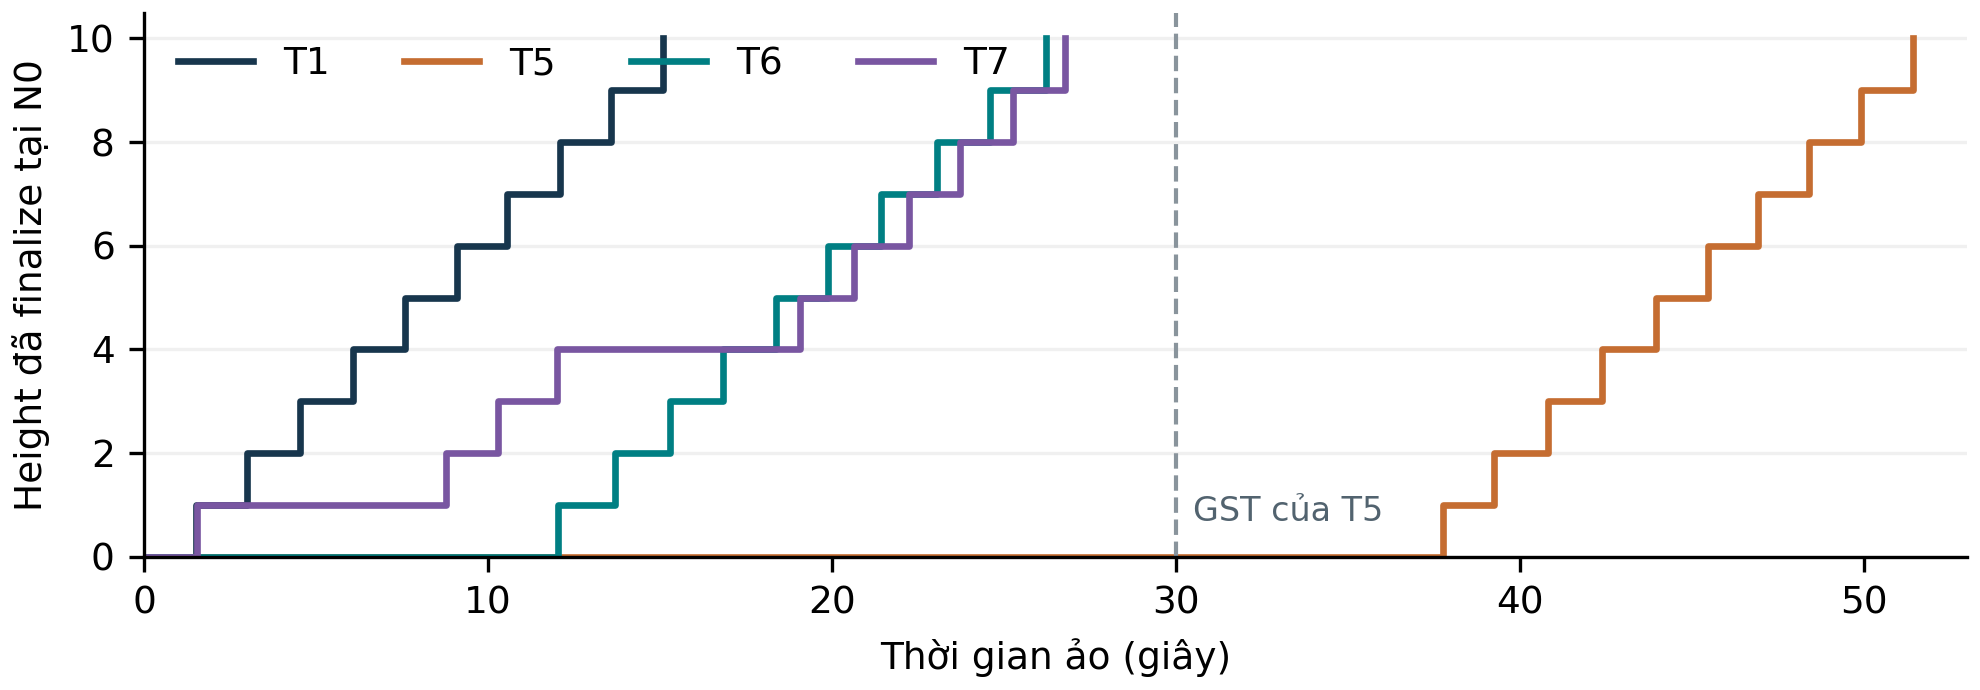
\includegraphics[width=0.94\linewidth]{report/figures/finalization.png}
\end{center}
\figcap{Hình 3. Tiến độ tại N0: T5 cần 51.464 s để toàn bộ node đúng đạt đích, so với 15.153 s ở T1. Đường nét đứt chỉ GST của T5; không phải một mốc của ba ca còn lại.}

{\small
\textbf{Quan sát lỗi:} T3 ghi 596 BAD\_SIGNATURE và 27 WRONG\_DOMAIN; T4 có 10 REPLAYED\_TX; T7 có 304 CONFLICTING\_VOTE. T5 có 1133 DROP và 80 DUPLICATE\_VOTE; T6 có 1 DUPLICATE\_VOTE. Các REJECT này phản ánh guard đang hoạt động, không phải test thất bại. T1 vẫn có 4232 DUP do cùng message đi tới node qua nhiều đường gossip, dù Link không tiêm lỗi duplicate. X1 áp dụng 114 TX tại N0; chưa kết luận mọi TX đã sinh đều được đưa vào chain.

\textbf{T8 -- tính xác định.} Hai log seed 42 trùng toàn bộ byte theo test, cùng final state hash; seed 43 cho log khác. Bảng 2 ghi 12 ký tự đầu SHA-256 để nhận diện; đối chiếu thực tế dùng digest đầy đủ và log gốc.

\begin{tabularx}{\linewidth}{lYYY}
\toprule
\textbf{Ca} & \textbf{Seed 42 / lần 1} & \textbf{Seed 42 / lần 2} & \textbf{Seed 43}\\\midrule
T1 & \code{e12ad6b6d06a} & \code{e12ad6b6d06a} & \code{549f197d3714} \\
T7 & \code{75f109db69da} & \code{75f109db69da} & \code{685c50883b3f} \\
\bottomrule\end{tabularx}
\par
}
